\documentclass{article}
\usepackage{graphicx}
\usepackage{amsmath}
\usepackage{pgfplots}
\usepackage[margin=1.5cm]{geometry}
\usepackage{adjustbox}
\usepackage{hyperref}
\usepackage{cite}
\pgfplotsset{compat=1.17}

\title{Relatório atividade "Prática de alocação de memória"}
\author{Alisson Luis Cordeiro de Arruda}
\date{Setembro 2024}

\begin{document}
\maketitle

\section{Introdução}
Este relatório apresenta os resultados de um código em C++ desenvolvido para medir e analisar dados relacionados ao tempo de execução e à utilização de memória durante a alocação de grandes quantidades de dados. O objetivo é compreender como uma grande quantidade de dados simultaneos impactam o desempenho do sistema e otimizar o uso de memória.

\section{Metodologia}
O código foi projetado para medir o tempo de execução e a utilização de memória durante diversas operações. Foram utilizadas funções específicas para rastrear esses parâmetros, garantindo precisão nos resultados. As medições foram feitas em um ambiente controlado, utilizando um sistema operacional Windows.

\section{Resultados}
Os resultados das medições foram coletados e organizados em gráficos, conforme mostrado nas Figuras \ref{fig:tempo_execucao}, \ref{fig:diferenca_memoria} e \ref{fig:uso_memoria} Os gráfico ilustram o tempo de execução em relação ao número do teste, diferença de memoria gasta durante os testes e total de memoria gasta des do inicio do programa.

\begin{figure}[h]
\centering
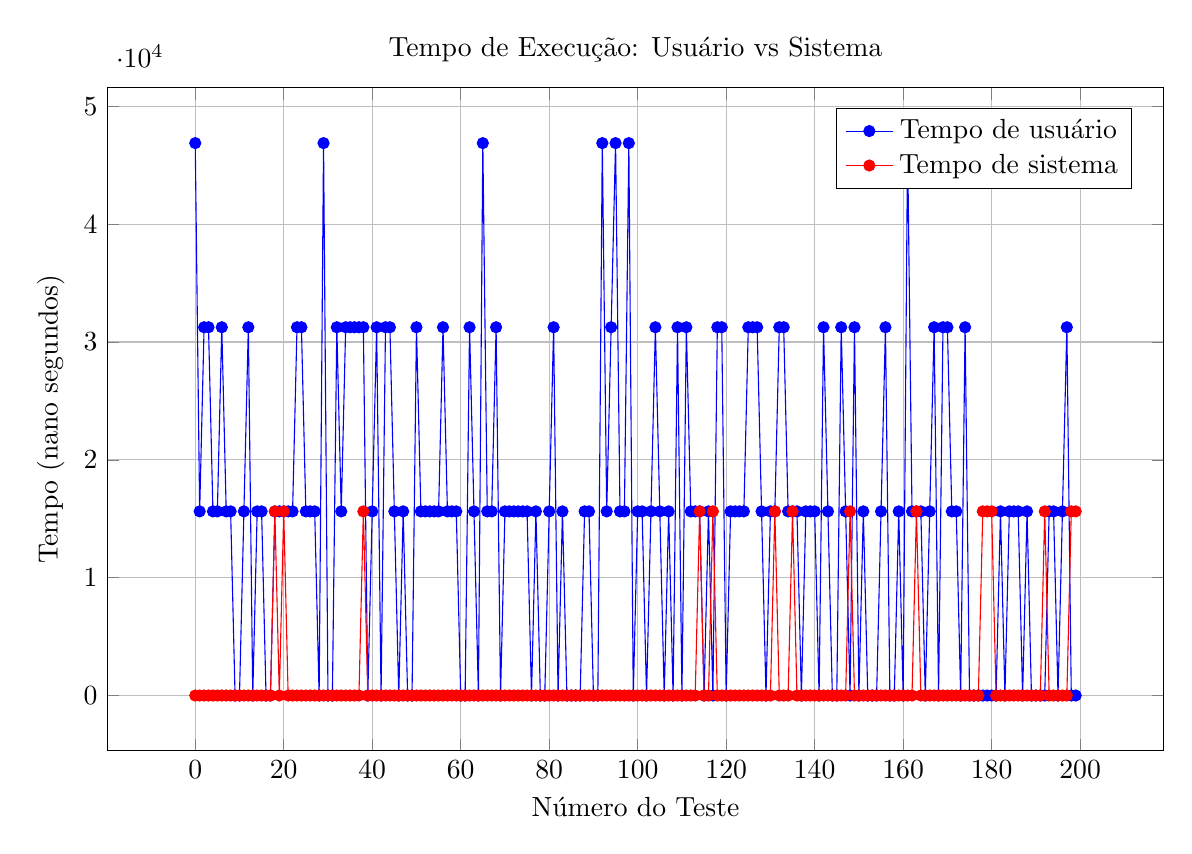
\begin{tikzpicture}
    \begin{axis}[
        width=15cm,
        height=10cm,
        title={Tempo de Execução: Usuário vs Sistema},
        xlabel={Número do Teste},
        ylabel={Tempo (nano segundos)},
        grid=major,
        legend pos=north east,
        yticklabel style={/pgf/number format/fixed},
        xticklabel style={/pgf/number format/fixed},
        cycle list name=color list]

    \addplot[color=blue, mark=*]
    coordinates{  (0, 46875) (1, 15625) (2, 31250) (3, 31250) (4, 15625) (5, 15625) (6, 31250) (7, 15625) (8, 15625) (9, 0) (10, 0) (11, 15625) (12, 31250) (13, 0) (14, 15625) (15, 15625) (16, 0) (17, 0) (18, 15625) (19, 15625) (20, 15625) (21, 15625) (22, 15625) (23, 31250) (24, 31250) (25, 15625) (26, 15625) (27, 15625) (28, 0) (29, 46875) (30, 0) (31, 0) (32, 31250) (33, 15625) (34, 31250) (35, 31250) (36, 31250) (37, 31250) (38, 31250) (39, 0) (40, 15625) (41, 31250) (42, 0) (43, 31250) (44, 31250) (45, 15625) (46, 0) (47, 15625) (48, 0) (49, 0) (50, 31250) (51, 15625) (52, 15625) (53, 15625) (54, 15625) (55, 15625) (56, 31250) (57, 15625) (58, 15625) (59, 15625) (60, 0) (61, 0) (62, 31250) (63, 15625) (64, 0) (65, 46875) (66, 15625) (67, 15625) (68, 31250) (69, 0) (70, 15625) (71, 15625) (72, 15625) (73, 15625) (74, 15625) (75, 15625) (76, 0) (77, 15625) (78, 0) (79, 0) (80, 15625) (81, 31250) (82, 0) (83, 15625) (84, 0) (85, 0) (86, 0) (87, 0) (88, 15625) (89, 15625) (90, 0) (91, 0) (92, 46875) (93, 15625) (94, 31250) (95, 46875) (96, 15625) (97, 15625) (98, 46875) (99, 0) (100, 15625) (101, 15625) (102, 0) (103, 15625) (104, 31250) (105, 15625) (106, 0) (107, 15625) (108, 0) (109, 31250) (110, 0) (111, 31250) (112, 15625) (113, 15625) (114, 15625) (115, 0) (116, 15625) (117, 0) (118, 31250) (119, 31250) (120, 0) (121, 15625) (122, 15625) (123, 15625) (124, 15625) (125, 31250) (126, 31250) (127, 31250) (128, 15625) (129, 0) (130, 15625) (131, 15625) (132, 31250) (133, 31250) (134, 15625) (135, 15625) (136, 15625) (137, 0) (138, 15625) (139, 15625) (140, 15625) (141, 0) (142, 31250) (143, 15625) (144, 0) (145, 0) (146, 31250) (147, 15625) (148, 0) (149, 31250) (150, 0) (151, 15625) (152, 0) (153, 0) (154, 0) (155, 15625) (156, 31250) (157, 0) (158, 0) (159, 15625) (160, 0) (161, 46875) (162, 15625) (163, 15625) (164, 15625) (165, 0) (166, 15625) (167, 31250) (168, 0) (169, 31250) (170, 31250) (171, 15625) (172, 15625) (173, 0) (174, 31250) (175, 0) (176, 0) (177, 0) (178, 0) (179, 0) (180, 0) (181, 0) (182, 15625) (183, 0) (184, 15625) (185, 15625) (186, 15625) (187, 0) (188, 15625) (189, 0) (190, 0) (191, 0) (192, 0) (193, 15625) (194, 15625) (195, 0) (196, 15625) (197, 31250) (198, 0) (199, 0) };

    \addplot[color=red, mark=*]
    coordinates{ (0, 0) (1, 0) (2, 0) (3, 0) (4, 0) (5, 0) (6, 0) (7, 0) (8, 0) (9, 0) (10, 0) (11, 0) (12, 0) (13, 0) (14, 0) (15, 0) (16, 0) (17, 0) (18, 15625) (19, 0) (20, 15625) (21, 0) (22, 0) (23, 0) (24, 0) (25, 0) (26, 0) (27, 0) (28, 0) (29, 0) (30, 0) (31, 0) (32, 0) (33, 0) (34, 0) (35, 0) (36, 0) (37, 0) (38, 15625) (39, 0) (40, 0) (41, 0) (42, 0) (43, 0) (44, 0) (45, 0) (46, 0) (47, 0) (48, 0) (49, 0) (50, 0) (51, 0) (52, 0) (53, 0) (54, 0) (55, 0) (56, 0) (57, 0) (58, 0) (59, 0) (60, 0) (61, 0) (62, 0) (63, 0) (64, 0) (65, 0) (66, 0) (67, 0) (68, 0) (69, 0) (70, 0) (71, 0) (72, 0) (73, 0) (74, 0) (75, 0) (76, 0) (77, 0) (78, 0) (79, 0) (80, 0) (81, 0) (82, 0) (83, 0) (84, 0) (85, 0) (86, 0) (87, 0) (88, 0) (89, 0) (90, 0) (91, 0) (92, 0) (93, 0) (94, 0) (95, 0) (96, 0) (97, 0) (98, 0) (99, 0) (100, 0) (101, 0) (102, 0) (103, 0) (104, 0) (105, 0) (106, 0) (107, 0) (108, 0) (109, 0) (110, 0) (111, 0) (112, 0) (113, 0) (114, 15625) (115, 0) (116, 0) (117, 15625) (118, 0) (119, 0) (120, 0) (121, 0) (122, 0) (123, 0) (124, 0) (125, 0) (126, 0) (127, 0) (128, 0) (129, 0) (130, 0) (131, 15625) (132, 0) (133, 0) (134, 0) (135, 15625) (136, 0) (137, 0) (138, 0) (139, 0) (140, 0) (141, 0) (142, 0) (143, 0) (144, 0) (145, 0) (146, 0) (147, 0) (148, 15625) (149, 0) (150, 0) (151, 0) (152, 0) (153, 0) (154, 0) (155, 0) (156, 0) (157, 0) (158, 0) (159, 0) (160, 0) (161, 0) (162, 0) (163, 15625) (164, 0) (165, 0) (166, 0) (167, 0) (168, 0) (169, 0) (170, 0) (171, 0) (172, 0) (173, 0) (174, 0) (175, 0) (176, 0) (177, 0) (178, 15625) (179, 15625) (180, 15625) (181, 0) (182, 0) (183, 0) (184, 0) (185, 0) (186, 0) (187, 0) (188, 0) (189, 0) (190, 0) (191, 0) (192, 15625) (193, 0) (194, 0) (195, 0) (196, 0) (197, 0) (198, 15625) (199, 15625) };

    \addlegendentry{Tempo de usuário}
    \addlegendentry{Tempo de sistema}

    \end{axis}
\end{tikzpicture}
\caption{Gráfico de Tempo de Execução}
\label{fig:tempo_execucao}
\end{figure}

\section{Medição de Memória}
A seção a seguir apresenta os gráficos referentes à medição de memória do código. O gráfico abaixo ilustra a memoria gasta durante cada caso de teste, o outro gráfico demonstra a quantidade de memoria gasta ao decorrer do programa.
\begin{figure}[!h]
    \centering
    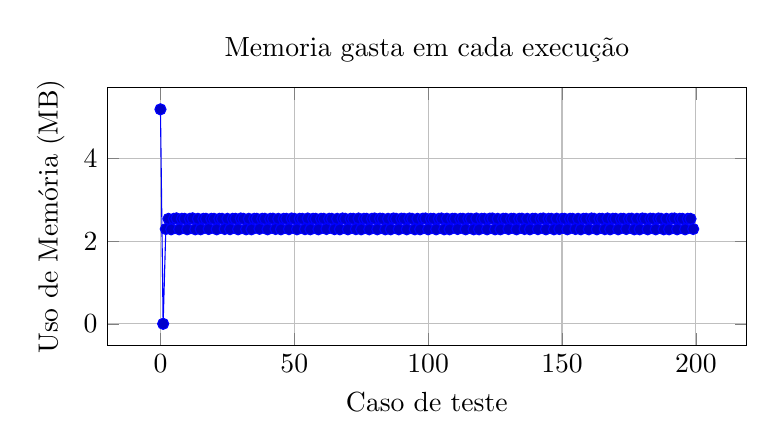
\begin{tikzpicture}
        \begin{axis}[
            title={Memoria gasta em cada execução},
            xlabel={Caso de teste},
            ylabel={Uso de Memória (MB)},
            grid=major,
            legend pos=outer north east,
            width=0.8\textwidth, 
            height=0.4\textwidth 
        ]
        % Adicione os dados do gráfico aqui, por exemplo:
        \addplot coordinates {(0, 5.1875) (1, 0) (2, 2.29297) (3, 2.53906) (4, 2.28516) (5, 2.53906) (6, 2.55078) (7, 2.28516) (8, 2.53906) (9, 2.53906) (10, 2.28516) (11, 2.53906) (12, 2.55078) (13, 2.28516) (14, 2.53906) (15, 2.28516) (16, 2.53906) (17, 2.53906) (18, 2.29297) (19, 2.53906) (20, 2.53906) (21, 2.28516) (22, 2.53906) (23, 2.53906) (24, 2.29297) (25, 2.53906) (26, 2.28906) (27, 2.53906) (28, 2.53906) (29, 2.28516) (30, 2.54688) (31, 2.53906) (32, 2.28516) (33, 2.53906) (34, 2.28516) (35, 2.53906) (36, 2.53906) (37, 2.29688) (38, 2.53906) (39, 2.53906) (40, 2.28516) (41, 2.53906) (42, 2.54297) (43, 2.29297) (44, 2.53906) (45, 2.28516) (46, 2.53906) (47, 2.53906) (48, 2.28906) (49, 2.54688) (50, 2.53906) (51, 2.28516) (52, 2.53906) (53, 2.53906) (54, 2.28906) (55, 2.54688) (56, 2.28516) (57, 2.53906) (58, 2.53906) (59, 2.28516) (60, 2.53906) (61, 2.53906) (62, 2.29297) (63, 2.53906) (64, 2.53906) (65, 2.28906) (66, 2.53906) (67, 2.28516) (68, 2.54688) (69, 2.53906) (70, 2.28516) (71, 2.53906) (72, 2.53906) (73, 2.28906) (74, 2.54688) (75, 2.28516) (76, 2.53906) (77, 2.53906) (78, 2.28516) (79, 2.53906) (80, 2.54688) (81, 2.28516) (82, 2.54297) (83, 2.53906) (84, 2.28516) (85, 2.53906) (86, 2.28516) (87, 2.54688) (88, 2.53906) (89, 2.28516) (90, 2.54297) (91, 2.53906) (92, 2.28516) (93, 2.54688) (94, 2.53906) (95, 2.28516) (96, 2.53906) (97, 2.28516) (98, 2.54297) (99, 2.54688) (100, 2.28516) (101, 2.53906) (102, 2.53906) (103, 2.28516) (104, 2.53906) (105, 2.54688) (106, 2.28516) (107, 2.54297) (108, 2.28516) (109, 2.53906) (110, 2.53906) (111, 2.29297) (112, 2.53906) (113, 2.53906) (114, 2.28516) (115, 2.54297) (116, 2.53906) (117, 2.28516) (118, 2.54688) (119, 2.28516) (120, 2.53906) (121, 2.53906) (122, 2.28516) (123, 2.54297) (124, 2.54688) (125, 2.28516) (126, 2.53906) (127, 2.28516) (128, 2.53906) (129, 2.53906) (130, 2.29297) (131, 2.53906) (132, 2.53906) (133, 2.28516) (134, 2.53906) (135, 2.54297) (136, 2.29297) (137, 2.53906) (138, 2.28516) (139, 2.53906) (140, 2.53906) (141, 2.28906) (142, 2.53906) (143, 2.54688) (144, 2.28516) (145, 2.53906) (146, 2.53906) (147, 2.28516) (148, 2.54297) (149, 2.29297) (150, 2.53906) (151, 2.53906) (152, 2.28516) (153, 2.53906) (154, 2.53906) (155, 2.29297) (156, 2.53906) (157, 2.28516) (158, 2.53906) (159, 2.53906) (160, 2.28516) (161, 2.54688) (162, 2.53906) (163, 2.28516) (164, 2.53906) (165, 2.53906) (166, 2.28906) (167, 2.54688) (168, 2.28516) (169, 2.53906) (170, 2.53906) (171, 2.28516) (172, 2.53906) (173, 2.53906) (174, 2.29297) (175, 2.53906) (176, 2.54297) (177, 2.28516) (178, 2.53906) (179, 2.28516) (180, 2.54688) (181, 2.53906) (182, 2.28516) (183, 2.54297) (184, 2.53906) (185, 2.28516) (186, 2.54688) (187, 2.53906) (188, 2.28516) (189, 2.53906) (190, 2.28516) (191, 2.54297) (192, 2.54688) (193, 2.28516) (194, 2.53906) (195, 2.53906) (196, 2.28516) (197, 2.53906) (198, 2.53906) (199, 2.29297)};

        \end{axis}
    \end{tikzpicture}
    \caption{Gráfico de memória: Por execução}
    \label{fig:diferenca_memoria}
\end{figure}

\begin{figure}[!h]
    \centering
    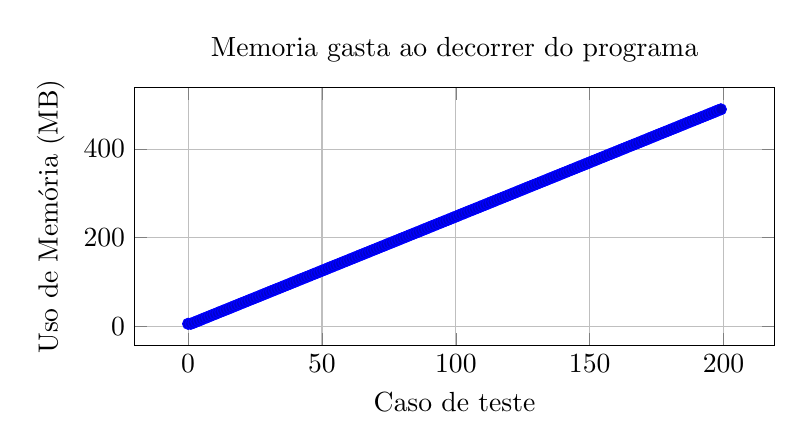
\begin{tikzpicture}
        \begin{axis}[
            title={Memoria gasta ao decorrer do programa},
            xlabel={Caso de teste},
            ylabel={Uso de Memória (MB)},
            grid=major,
            legend pos=outer north east,
            width=0.8\textwidth,
            height=0.4\textwidth
        ]
        
        \addplot coordinates { (0, 5.1875) (1, 5.27344) (2, 7.56641) (3, 10.1055) (4, 12.3906) (5, 14.9297) (6, 17.4805) (7, 19.7656) (8, 22.3047) (9, 24.8438) (10, 27.1289) (11, 29.668) (12, 32.2188) (13, 34.5039) (14, 37.043) (15, 39.3281) (16, 41.8672) (17, 44.4102) (18, 46.7031) (19, 49.2422) (20, 51.7812) (21, 54.0664) (22, 56.6055) (23, 59.1445) (24, 61.4375) (25, 63.9766) (26, 66.2656) (27, 68.8047) (28, 71.3438) (29, 73.6289) (30, 76.1758) (31, 78.7148) (32, 81) (33, 83.543) (34, 85.8281) (35, 88.3672) (36, 90.9062) (37, 93.1992) (38, 95.7383) (39, 98.2773) (40, 100.566) (41, 103.105) (42, 105.645) (43, 107.938) (44, 110.477) (45, 112.762) (46, 115.305) (47, 117.844) (48, 120.129) (49, 122.676) (50, 125.215) (51, 127.5) (52, 130.039) (53, 132.582) (54, 134.867) (55, 137.414) (56, 139.699) (57, 142.238) (58, 144.777) (59, 147.066) (60, 149.605) (61, 152.145) (62, 154.438) (63, 156.977) (64, 159.516) (65, 161.801) (66, 164.34) (67, 166.625) (68, 169.172) (69, 171.711) (70, 173.996) (71, 176.539) (72, 179.078) (73, 181.363) (74, 183.91) (75, 186.449) (76, 188.734) (77, 191.273) (78, 193.559) (79, 196.102) (80, 198.648) (81, 200.934) (82, 203.473) (83, 206.012) (84, 208.297) (85, 210.836) (86, 213.121) (87, 215.668) (88, 218.211) (89, 220.496) (90, 223.035) (91, 225.574) (92, 227.859) (93, 230.406) (94, 232.945) (95, 235.23) (96, 237.773) (97, 240.059) (98, 242.598) (99, 245.145) (100, 247.43) (101, 249.969) (102, 252.508) (103, 254.793) (104, 257.336) (105, 259.883) (106, 262.168) (107, 264.707) (108, 266.992) (109, 269.531) (110, 272.07) (111, 274.363) (112, 276.902) (113, 279.445) (114, 281.73) (115, 284.27) (116, 286.809) (117, 289.094) (118, 291.641) (119, 293.926) (120, 296.465) (121, 299.008) (122, 301.293) (123, 303.832) (124, 306.379) (125, 308.664) (126, 311.203) (127, 313.742) (128, 316.027) (129, 318.574) (130, 320.867) (131, 323.406) (132, 325.945) (133, 328.23) (134, 330.77) (135, 333.312) (136, 335.605) (137, 338.145) (138, 340.43) (139, 342.969) (140, 345.508) (141, 347.797) (142, 350.336) (143, 352.883) (144, 355.168) (145, 357.707) (146, 360.246) (147, 362.531) (148, 365.074) (149, 367.367) (150, 369.906) (151, 372.445) (152, 374.73) (153, 377.27) (154, 379.812) (155, 382.105) (156, 384.645) (157, 387.184) (158, 389.469) (159, 392.008) (160, 394.293) (161, 396.84) (162, 399.379) (163, 401.664) (164, 404.203) (165, 406.742) (166, 409.027) (167, 411.574) (168, 413.859) (169, 416.398) (170, 418.938) (171, 421.223) (172, 423.766) (173, 426.305) (174, 428.598) (175, 431.137) (176, 433.676) (177, 435.961) (178, 438.5) (179, 440.785) (180, 443.332) (181, 445.871) (182, 448.16) (183, 450.699) (184, 453.238) (185, 455.523) (186, 458.07) (187, 460.609) (188, 462.895) (189, 465.434) (190, 467.723) (191, 470.262) (192, 472.809) (193, 475.094) (194, 477.633) (195, 480.172) (196, 482.457) (197, 485) (198, 487.539) (199, 489.832)};
        
        \end{axis}
    \end{tikzpicture}
    \caption{Gráfico de Memória: total}
    \label{fig:uso_memoria}
\end{figure}

\section{Endereços de Memória}
Nesta seção, discutimos os endereços de memória observados durante as medições. Os endereços de memória são referências numéricas a locais específicos na memória do computador onde os dados são armazenados. Durante a execução do código, foi possível rastrear os endereços utilizados para alocar variáveis e estruturas de dados.

Os endereços de memória são fundamentais para entender como a memória é gerenciada e utilizada pelo programa. O monitoramento desses endereços ajuda a identificar possíveis vazamentos de memória ou acessos indevidos. Abaixo estão os endereços coletados durante as medições:

\begin{itemize}
    \item Endereço 1: 2457252622408
    \item Endereço 2: 2457252622408
    \item ...
    \item Endereço 200: 2457252622408
\end{itemize}

Observamos que em todos os casos de teste os endereços de memoria continuam os mesmos, isso se da pelo fato de os testes terem sidos feitos em um hardware com bastante memoria ram disponivel, evitando que os dados tenham que ser movidos para outro endereço.

\section{Dificuldades}
Durante o processo de criação do codigo, foram vistas diversas dificuldades de entendimento da atividade, a partir de uma revisão aprofundada do conteudo e estudos feitos com auxilio de videos e sites, foi possivel desenvolver o projeto, atingindo o objetivo estimado.

\section{Conclusões}
O codigo demora em media 12-18 segundos para executar completamente, "graças a deus" o codigo não vaza memoria, deleta todos os dados perfeitamente e não aloca itens desnecessarios, o objetivo da atividade foi atingido e todos os requisitos foram cumpridos. Infelizmente o codigo foi feito via windows então pode não rodar em um ambiente linux devido a falta de algumas bibliotecas.

\section{Referências}
\begin{enumerate}
    \item ChatGPT. "Modelo de linguagem da OpenAI." Disponível em: \url{https://www.openai.com/chatgpt}
    \item Playlist YouTube. "Estrutura de dados" Disponível em: \url{https://www.youtube.com/watch?v=ucupombJuUM&list=PL3ZslI15yo2r-gHJtjORRMRKMSNRpf7u5}
    \item Medium. "Programação e exemplos de codigo c++ em: \url{https://medium.com}
\end{enumerate}

\end{document}
